\documentclass[12pt]{article}
\usepackage{amsmath}
\usepackage[T1]{fontenc}
\usepackage{graphicx}
\usepackage{amsfonts}
\newcommand{\abs}[1]{\left| #1 \right|}
\title{MDL 5 7.11}
\author{Dominik Szczepaniak}
\begin{document}

\maketitle
Zrobione:
\begin{tabular}{|| c c c c c c c c c c c||}
    \hline
    2 & 4 & 6 & 7D & 8 & 9 & 10 & 11 & 12  \\
    \hline
    Y & Y & Y & N & Y & Y & Y & Y & Y
\end{tabular}

\bgroup\obeylines

\section{Zadanie 2}
Załóżmy, że mamy już n linii i chcemy podzielić płaszczyzne kolejną linią na jak najwięcej części. Wtedy w najlepszym wypadku przetniemy każdą z n-1 linii w nowym miejscu przecięcia. Przetniemy więc najpierw pierwszy region (zanim jakąkolwiek linie) na dwa, a później dla każdej przeciętej linii będziemy dzielić jakiś region na dwa. 
W takim razie mamy 
$p_n$ = $p_{n-1} + 2*(n-1) + 1$
$p_n - p_{n-1} + 2n-2+1= 0$
$p_n - p_{n-1} + 2n - 1 = 0$
$p_{n+1} - p_{n} + 2n + 1 = 0$
$p_{n+1} - p_{n} => (E-1)$
$2n+1 => (E-1)^2$
$(E-1)^3<p_n> = 0$
$p_n = \alpha * 1^n + \beta * n * 1^n + \gamma * n^2 * 1^n = \alpha + n\beta + n^2\gamma$
$p_0 = 1 = \alpha$
$p_1 = 2 = \alpha + \beta + \gamma$
$p_2 = 4 = \alpha + 2\beta + 4\gamma$
$\newline$
$1+\beta+\gamma = 2$
$\beta = 1 - \gamma$
$\newline$
$1 + 2 - 2\gamma + 4\gamma = 4$
$2\gamma = 1$
$\gamma = \frac{1}{2}$
$\beta = \frac{1}{2}$
$p_n = 1 + \frac{n}{2} + \frac{n^2}{2}$




\section{Zadanie 4}
Podpunkt a
a0 = 1
a1 = 1
$a2 = \sqrt{1+1} = \sqrt{2}$
$a3 = \sqrt{2+1} = \sqrt{3}$
$a4 = \sqrt{2+3} = \sqrt{5}$
$a_n = \sqrt{fib(n+1)}$
Z pdf'a wiemy, ze 
$Fib(n) = \frac{1}{\sqrt{5}}*(\frac{1+\sqrt{5}}{2})^n - \frac{1}{\sqrt{5}}*(\frac{1-\sqrt{5}}{2})^n$
W takim razie 
$a_n = \sqrt{\frac{1}{\sqrt{5}}*(\frac{1+\sqrt{5}}{2})^{n+1} - \frac{1}{\sqrt{5}}*(\frac{1-\sqrt{5}}{2})^{n+1}}$

Podpunkt b 
$b_{n+1} = \sqrt{{b_n}^2 + 3}, b_0 = 8$
$b_{n+1} = \abs{\sqrt{{b_{n}}^2 + 3}} = \abs{\sqrt{\abs{\sqrt{b_{n-1}^2 + 3}}^2 + 3}} = \abs{\sqrt{b_{n-1}^2 + 3 + 3}} = \abs{\sqrt{\abs{\sqrt{b_{n-2}^2 + 3}}^2 + 3 + 3}} = \abs{\sqrt{b_{n-2}^2 + 3 + 3 + 3}} = \abs{\sqrt{b_{n-3}^2 + 3 + 3 + 3 + 3}} = \abs{\sqrt{b_{n-4}^2 + 3 + 3 + 3 + 3 + 3}} = \abs{\sqrt{ b_0^2 + 3n }} = \abs{\sqrt{ 64 + 3n }}$

Podpunkt c 
$c_{n+1} = (n+1)c_n + (n^2+n)c_{n-1}, c0 = 0, c1 = 1$
$c_2 = 2*1 + 2*0 = 2$
$c_3 = 3*2 + 6*1 = 12$
$c_4 = 4*12 + 12*2 = 72$
$c_5 = 5*72 + 20*12 = 600$
$\vdots$
$c_n = n! * F_n$

Dla $n=0$ mamy 
$c_0 = 0! * fib{0} = 1*0 = 0$, czyli sie zgadza
Załóżmy, że dla $n$ zachodzi, wtedy chcemy pokazać indukcyjnie, że dla $n+1$ też zachodzi:
$c_{n+1} = (n+1)c_n + (n^2+n)c_{n-1} = (n+1) * n! * F_n + (n^2+n) * (n-1)! * F_{n-1} = (n+1) * n! * F_n + (n+1) * n * (n-1)! * F_{n-1} = (n+1)! * F_n + (n+1)! * F_{n-1} = (n+1)!(F_n + F_n-1) = (n+1)! * F_{n+1}$ 
Czyli się zgadza

\section{Zadanie 6}
Chcemy pokazać, że $a * (a+1) * (a+2) * \dots * (a+k-1)$ dzieli się przez $k!$
$\binom{n}{k} = \frac{n*(n-1)*\dots*(n-k+1)}{k*(k-1)*\dots*1}$
Mamy w takim razie góre która wygląda jak nasz iloczyn. Dzieli się przez k!, więc chcemy pomnożyć i mamy to samo.
$a * (a+1) * (a+2) * \dots * (a+k-1) = \binom{a+k-1}{k} * k!$
$\binom{a+k-1}{k} \in \mathbb{Z}$ 
więc dzieli się przez k!

\section{Zadanie 7}
$D_0 = 1$
$D_1 = 0$

$D_{n+1} = n*(D_n + D_{n-1})$
$D_{n+1} - nD_n - nD_{n-1} = 0$
$(E^2 - nE - n)*<D_n> = 0$
$(E - (\frac{1}{2}*(n-\sqrt{n}*\sqrt{n+4})))(E-(\frac{1}{2}*(n+\sqrt{n}*\sqrt{n+4})))*<D_n> = 0$
$D_n = \alpha * (\frac{1}{2}*(n-\sqrt{n}*\sqrt{n+4}))^n + \beta * (\frac{1}{2}*(n+\sqrt{n}*\sqrt{n+4}))^n$
$D_0 = 1 = \alpha + \beta => \alpha = 1 - \beta$
$D_1 = 0 = (1 - \beta)*(\frac{1}{2}*(1-\sqrt{1}*\sqrt{5})) + \beta * (\frac{1}{2}*(1+\sqrt{1}*\sqrt{5}))$
$ = (\frac{1}{2}*(1-1*\sqrt{5})) - \beta*(\frac{1}{2}*(1-1*\sqrt{5})) + \beta * (\frac{1}{2}*(1+1*\sqrt{5}))$ 
$= \frac{1-\sqrt{5}}{2} - \beta*(\frac{1-\sqrt{5}}{2}) + \beta*\frac{1+\sqrt{5}}{2} =$
$\beta(- \frac{1-\sqrt{5}}{2} + \frac{1+\sqrt{5}}{2}) + \frac{1-\sqrt{5}}{2} = \beta(\sqrt{5}) + \frac{1+\sqrt{5}}{2}$
$\beta(\sqrt{5}) + \frac{1+\sqrt{5}}{2} = 0$
$\beta = \frac{1+\sqrt{5}}{2*\sqrt{5}} = \frac{\sqrt{5} + 5}{10}$

$\beta = \frac{1}{2} - \frac{1}{2*\sqrt{5}}$

$\beta = \frac{1}{2} - \frac{25}{12*\sqrt{21}}$

$\alpha = \frac{1}{2} + \frac{1}{2*\sqrt{5}}$

$D_n = \frac{1}{2} + \frac{1}{2*\sqrt{5}} * (\frac{1}{2}*(n-\sqrt{n}*\sqrt{n+4}))^n + \frac{1}{2} - \frac{1}{2*\sqrt{5}} * (\frac{1}{2}*(n+\sqrt{n}*\sqrt{n+4}))^n$

\section{Zadanie 8}
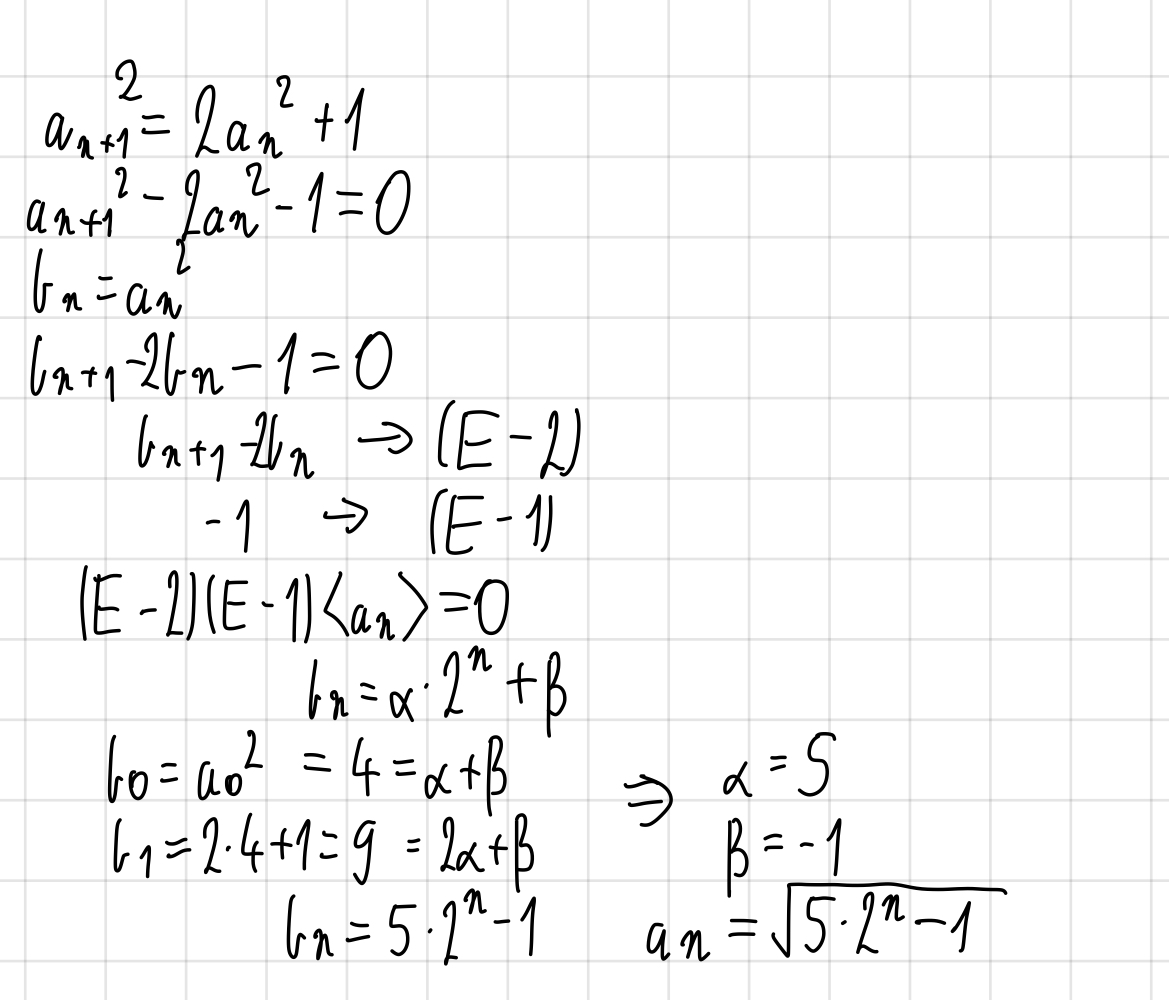
\includegraphics[width=120mm]{zad8}

\section{Zadanie 9}

Wyraz złożony z 0 liter zawiera 0 liter a, a więc parzystą ilość także $a_0 = 1$.
Dla wyrazów złożonych z 1 litery mamy 24 wyrazy bez litery a. Czyli $a_1 = 24$
Dla ogólnego przypadku n liter:
$a_n = 24*a_{n-1} + (25^{n-1} - a_{n-1}) = 25^{n-1} + 23*a_{n-1}$
$24*a_{n-1}$ - a nie będzie ostatnią literą, więc rozpatrujemy ciągi o długości n-1 zawierające parzystą liczbę wystąpień a 
$(25^{n-1} - a_{n-1})$ - a będzie ostatnią literą, więc rozpatrujemy ciągi długości n-1 zawierające nieparzystą liczbę a
$\newline$
$a_n = 25^{n-1} + 23*a_{n-1}$
$a_n - 23*a_{n-1} - 25^{n-1} = 0$
$a_{n+1} - 23*a_n - 25^n = 0$
$a_{n+1} - 23*a_n => (E - 23)$
$-25^{n} => (E-25)$
$(E-23)*(E-25)<a_n> = 0$
$a_n = \alpha * 23^n + \beta * 25^n$
$\newline$
$a_0 = 1 = \alpha + \beta$
$a_1 = 24 = \alpha * 23^1 + 25^1 *\beta$
$\newline$
$\alpha = 1 - \beta$
$24 = 23 - 23\beta + 25\beta$
$1 = 2\beta$
$\beta = \frac{1}{2}$
$\alpha = \frac{1}{2}$
$a_n = \frac{1}{2}23^n + 25^n\frac{1}{2}$


\section{Zadanie 10}
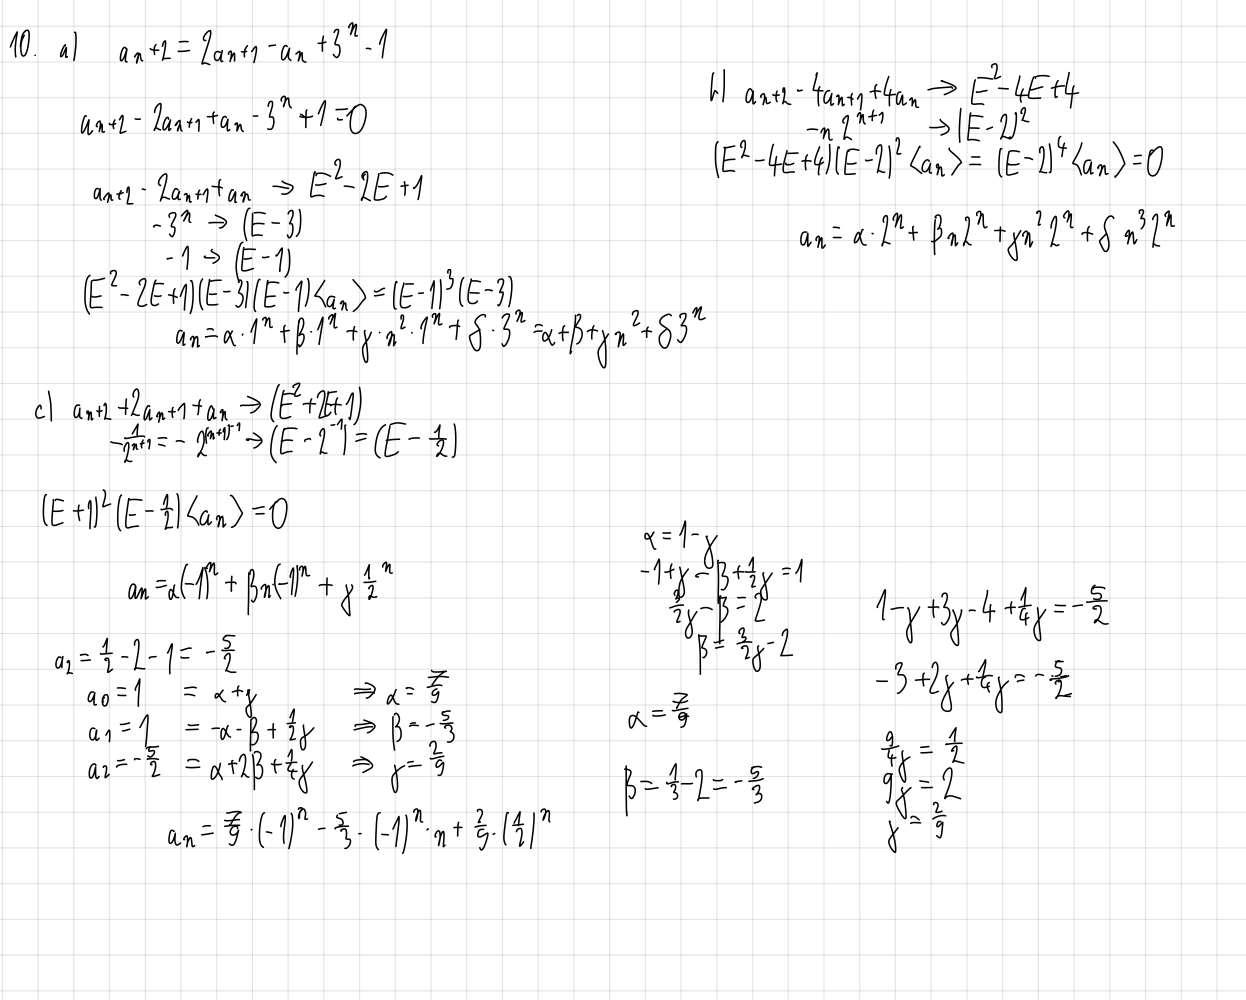
\includegraphics[width=180mm]{zad10}
\section{Zadanie 11}
$c_0 = 1$
Jeśli chcemy nie mieć dwóch następujących po sobie zer lub jedynek, to poprzedni ciąg możemy przedłużyć jedną z dwóch cyfr, bo ta trzecia będzie kolejną taką samą, jeśli skończyliśmy ostatni ciąg na 0 lub 1 albo możemy przedłużyć o 2 jeśli skończyliśmy na 2.
$\newline$
dp[i][0] - kończone na 0/1 
dp[i][1] - kończone na 2
$\newline$
dp[1][0] = 2
dp[1][1] = 1
$\newline$
dp[i+1][0] = dp[i][0] + 2*dp[i][1]
dp[i+1][1] = (dp[i][0] + dp[i][1])
$\newline$
dp[i][0] = dp[i-1][0] + 2*dp[i-1][1]
dp[i][1] = (dp[i-1][0] + dp[i-1][1])
$\newline$
dp[i+1][0] = dp[i-1][0] + 2*dp[i-1][1] + 2dp[i-1][0] + 2dp[i-1][1] = 3dp[i-1][0] + 4dp[i-1][1]
dp[i+1][1] = dp[i-1][0] + 2*dp[i-1][1] + dp[i-1][0] + dp[i-1][1] = 2dp[i-1][0] + 3dp[i-1][1]
$\newline$
dp[i+2][0] = dp[i+1][0] + 2*dp[i+1][1]
dp[i+1][1] = dp[i+1][0] + dp[i+1][1]
$\newline$
dp[i+2][0] = 7dp[i-1][0] + 10dp[i-1][1]
dp[i+2][1] = 5dp[i-1][0] + 7dp[i-1][1]
$\newline$
dp[i] = 2dp[i-1][0] + 3dp[i-1][1] 
dp[i+1] = 5dp[i-1][0] + 7dp[i-1][1] 
dp[i+2] = 12dp[i-1][0] + 17dp[i-1][1] 
dp[i+3] = 29dp[i-1][0] + 41dp[i-1][1] 
$\newline$
Niech i = 2
dp[0] = 1
dp[1] = 2 + 1 = 3
dp[2] = 4 + 3 = 7
dp[3] = 10 + 7 = 17 
dp[4] = 24 + 17 = 41 
dp[5] = 58 + 41 = 99
$\newline$
Zauważmy, że dp[i] = 2*dp[i-1] + dp[i-2]
W takim razie 
Dla n mamy 
$c_n = 2c_{n-1} + c_{n-2}$
$c_{n+1} - 2c_n - c_{n-1} = 0$
$(E^2 - 2E - 1)<c_n> = 0$
$(E-1+\sqrt{2})(E-1-\sqrt{2})<c_n> = 0$
$c_n = \alpha*(1-\sqrt{2})^n + \beta*(1+\sqrt{2})^n$
$c_0 = 1 = \alpha + \beta => \alpha = 1 - \beta$
$c_1 = 3 = \alpha*(1-\sqrt{2}) + \beta*(1+\sqrt{2})$
$\newline$
$\alpha*(1-\sqrt{2}) + \beta*(1+\sqrt{2}) = 3$
$(1 - \beta)*(1-\sqrt{2}) + \beta*(1+\sqrt{2}) = 3$
$(1-\sqrt{2}) - \beta*(1-\sqrt{2}) + \beta*(1+\sqrt{2}) = 3$
$(1-\sqrt{2}) - \beta + \beta \sqrt{2} + \beta + \beta \sqrt{2} = 3$
$(1-\sqrt{2}) + 2\beta \sqrt{2} = 3$
$2\beta \sqrt{2} = 3 - 1 + \sqrt{2}$
$2\beta \sqrt{2} = 2 + \sqrt{2}$
$2\beta = \frac{2\sqrt{2}}{2} + 1$
$\beta = \frac{\sqrt{2}}{2} + \frac{1}{2}$
$\alpha = 1 - \frac{\sqrt{2}}{2} - \frac{1}{2} = \frac{1}{2} - \frac{\sqrt{2}}{2}$

$c_n = (\frac{1}{2} - \frac{\sqrt{2}}{2}) * (1-\sqrt{2})^n + (\frac{\sqrt{2}}{2} + \frac{1}{2})*(1+\sqrt{2})^n$


\section{Zadanie 12}
$a) 1*4^{n-1}$
$b) 2^n$
$c) 4^{n-2}$
$d) 3^n$
$e) \lfloor 4^{n-4} \rfloor$

\egroup
\end{document}